\documentclass[conference]{IEEEtran}
\IEEEoverridecommandlockouts
% The preceding line is only needed to identify funding in the first footnote. If that is unneeded, please comment it out.
\usepackage{cite}
\usepackage{amsmath,amssymb,amsfonts}
\usepackage{algorithmic}
\usepackage{graphicx}
\usepackage{textcomp}
\usepackage{xcolor}
\def\BibTeX{{\rm B\kern-.05em{\sc i\kern-.025em b}\kern-.08em
    T\kern-.1667em\lower.7ex\hbox{E}\kern-.125emX}}
\begin{document}

\title{Classification of Brain Tumors by Image Processing and Ensemble Learning\\}

\author{\IEEEauthorblockN{1\textsuperscript{st} Hakan Tekgul}
\IEEEauthorblockA{\textit{Electrical and Computer Engineering} \\
\textit{Georgia Institute of Technology}\\
Metz, France \\
htekgul3@gatech.edu}
\and
\IEEEauthorblockN{2\textsuperscript{nd} Jad Sinno}
\IEEEauthorblockA{\textit{Electrical and Computer Engineering} \\
\textit{Georgia Institute of Technology}\\
Metz, France \\
jsinno3@gatech.edu}
\and
\IEEEauthorblockN{3\textsuperscript{rd} Madhur Gupta}
\IEEEauthorblockA{\textit{Electrical and Computer Engineering} \\
\textit{Georgia Institute of Technology}\\
Metz, France \\
mgupta325@gatech.edu}
}

\maketitle

\begin{abstract}
When diagnosed at a late stage, brain cancers and tumors provide very short life expectancy and a high mortality rate because of their aggressive nature. In order to diagnose and detect the tumor on the brain at the earliest stage possible, various medical imaging techniques such as Computed Tomography (CT) or Magnetic Resonance Imaging (MRI) are used. Unfortunately, the diagnosis and treatment of the tumor depends highly on the physician’s medical knowledge. Hence, many different systems have been proposed in the past decade to automatically detect brain tumors by using machine learning. One major problem with these approaches is the fact that they usually need lots of training data (MRI Scans).  

In this project, we detect brain tumors from MRI images with a limited amount of training data, around 120 images. Specifically, we use an ensemble learning approach that is based on Support Vector Machines (SVM). After applying image processing techniques such as low-pass filtering to all the images, the most common prediction from different SVM classifiers is chosen for a testing image. Validation accuracies are used to select the best image processing techniques and their optimal parameters. Our experimental results suggest that the Ensemble Classifier achieves an accuracy of 87\% with low time complexity.
\end{abstract}

\begin{IEEEkeywords}
Brain Tumor, Image Classification, Ensemble Learning, Medical Imaging, SVM
\end{IEEEkeywords}

\section{Introduction}\label{intro}
\subsection{Motivation}
% Explain the motivation behind project and goal of project
Brain cancers and tumors affect the life of humans negatively, as abnormal growth of brain cells damage the functioning of the brain and might even lead to death. With increased usage of cell phones, the incidence rate of brain tumors is predicted to rise rapidly[REF]. Furthermore, the mortality rate of brain cancers have also been increasing constantly in the past decade[REF]. In order to reduce the mortality rate and treat brain tumors, diagnosis should be done in the earliest stage possible. 

Medical imaging is used to diagnose and visualize different types of tumors in the human body. Various medical imaging techniques such as CT Scan, MRI, or X-Ray is used in hospitals for diagnosis. Magnetic Resonance Imaging (MRI) is generally used for brain tumor diagnosis as it shows the inside of the brain with contrast. With the use of MRI, brain tumors are identified as soon as possible by many physicians. However, some MRI scans are hard to read and there is a chance that physicians can make a mistake during diagnosis. When a physician decides that a tumor in the brain does not exist but in reality there is a tumor, a false negative diagnosis occurs and such diagnosis can be catastrophic for the patient. Hence, many different systems have been proposed in the past decade that automatically identifies brain tumors in an MRI scan. Even though most of these approaches have good accuracy and results, they usually need a huge number of training data and computation resources. Therefore, new approaches for brain tumor classification must be considered. 

In this work, we propose to detect brain tumors from MRI images with a limited amount of training data. Specifically, we use image processing and ensemble learning through Support Vector Machines (SVM) to classify whether an MRI scan has a tumor or not. Our main goal in this study is to maximize the classification accuracy and minimize the number of false negatives. We use different image processing techniques, inluding Low-Pass Filter (LPF), High-Pass Filter (HPF), Median Filter (MF), and Low-Pass - High-Pass Filter (LPF+HPF). Then, we apply different machine learning algorithms such as k-NN, SVM, and Neural Networks (NN). To summarize, we make three main contributions in this paper:
\begin{itemize}
  \item We apply different image filters to MRI scans and analyze the best processing technique for tumor detection.
  \item We experiments with three different machine learning algorithms and state their accuracy for differrent image processing techniques.
  \item We propose an ensemble learning approach that successfully identifies a tumor in the brain with a minimum number of false negatives. 
\end{itemize}
Our experimental results suggest that LPF+HPF is the best filter to use for tumor detection, with an average classification accuracy of 84\%. Additionaly, we observed that Support Vector Machines (SVM) gives the optimal results in terms of classification. Finally, our ensemble learning approach that is based on different filters and Support Vector Machines outputs a classification accuracy of 87\% and a 2\% false negative rate. 

\subsection{Related Work} 
% Discuss some related work. Provide around 5-6 projects about tumor classification and summarize their improvements/results
% DO NOT FORGET TO CITE

\section{Methodology}\label{method}
% Put the flowchart here 
\begin{figure}[h]
\centering
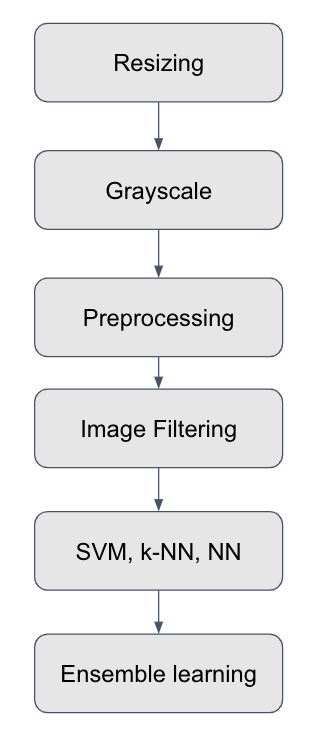
\includegraphics[scale=0.4]{flowchart}
\caption{Flowchart of the project that summarizes our process for our experiments.}
\end{figure}
% Explain our methodology behind the project
% Talk briefly about resizing and grayscale. Maybe put the graph on image sizes? 

For this project, we used an MRI Scan dataset that has a total of 255 images. The dataset is balanced, where there are 156 positive images and 99 negative images. From the 255 images, 70\% is used for training and 30\% is used for testing. After that, all the images are resized to a certain size through bicubic interpolation and each image is converted to grayscale. This was because the MRI scans usually consist of black and white pixels and RGB colors does not contribute to identification of tumors. Note that the methodology behind this project is shown in Figure 1.

\subsection{Image Preprocessing}
% Describe the equalization and contrast images

\subsection{Image Filtering}
% Describe and explain the different filters 

\subsection{Machine Learning}
% Briefly describe the machine learning algorithms 
After creating the contrasted, equalized versions of the dataset and applying different image filters, classification experiments are conducted by applying three different machine learning algorithms. As stated before, k-Nearest Neighbors (kNN), Support Vector Machines (SVM), and Artificial Neural Networks (NN) are applied on our data. k-NN is chosen because of its simplicity and the fact that our images are not that complex in nature. SVM, on the other hand, is selected as a machine learning algorithm because it can work very well with low amount of training data and it handles outliers very well. Finally, because image classification is usually done with Neural Networks, we chose NN as the last algorithm. 

% Cross validation
After choosing the algorithms, the dataset is split into training, validation, and testing. As stated before, 70\% of data is used for training and 30\% of training set is used for validation. Then, all the specified machine learning algorithms are applied to the training set and cross-validation approach is used to tune the parameters of each algorithm. After the optimization of the classifiers, accuracy results are collected for different classifiers, different image filters, and their different sigma values. Such results are presented in section 3. 

% Ensemble Learning
Finally, best 8 classifier/filter/sigma combinations that had the maximum but different accuracies are selected for ensemble learning. Ensemble learning is applied because some of the classifiers had overfitting and there was a need to generalize the data better. At the end, the most common prediction from the 8 classifiers is taken as the final result. In the case of a tie, the classifier predicts a positive instance to lower the number of false negatives.

\section{Experimental Results}\label{results}
% Provide experimental results here
% Provide 3 different tables --> cluster all k-NN results together into one table, same for SVM and NN
% Learning curves, validation curves
% Final Confusion Matrix 

\section{Analysis of Results}\label{analysis}
% Detailed analysis of all results and process
% Analyze the results for each filter, different sigma values, and for each ML algorithm
% Which image filter worked the best? 
% Which algorithm worked the best?
% How helpful was ensemble learning?
% Discuss false negatives and accuracy 

\section{Conclusion and Future Work}\label{conclusion}
% Briefly summarize main ideas of project
% Discuss future work such as tumor segmentation

\section*{Acknowledgment}

The preferred spelling of the word ``acknowledgment'' in America is without 
an ``e'' after the ``g''. Avoid the stilted expression ``one of us (R. B. 
G.) thanks $\ldots$''. Instead, try ``R. B. G. thanks$\ldots$''. Put sponsor 
acknowledgments in the unnumbered footnote on the first page.

\section*{References}

Please number citations consecutively within brackets \cite{b1}. The 
sentence punctuation follows the bracket \cite{b2}. Refer simply to the reference 
number, as in \cite{b3}---do not use ``Ref. \cite{b3}'' or ``reference \cite{b3}'' except at 
the beginning of a sentence: ``Reference \cite{b3} was the first $\ldots$''

Number footnotes separately in superscripts. Place the actual footnote at 
the bottom of the column in which it was cited. Do not put footnotes in the 
abstract or reference list. Use letters for table footnotes.

Unless there are six authors or more give all authors' names; do not use 
``et al.''. Papers that have not been published, even if they have been 
submitted for publication, should be cited as ``unpublished'' \cite{b4}. Papers 
that have been accepted for publication should be cited as ``in press'' \cite{b5}. 
Capitalize only the first word in a paper title, except for proper nouns and 
element symbols.

For papers published in translation journals, please give the English 
citation first, followed by the original foreign-language citation \cite{b6}.

\begin{thebibliography}{00}
\bibitem{b1} G. Eason, B. Noble, and I. N. Sneddon, ``On certain integrals of Lipschitz-Hankel type involving products of Bessel functions,'' Phil. Trans. Roy. Soc. London, vol. A247, pp. 529--551, April 1955.
\bibitem{b2} J. Clerk Maxwell, A Treatise on Electricity and Magnetism, 3rd ed., vol. 2. Oxford: Clarendon, 1892, pp.68--73.
\bibitem{b3} I. S. Jacobs and C. P. Bean, ``Fine particles, thin films and exchange anisotropy,'' in Magnetism, vol. III, G. T. Rado and H. Suhl, Eds. New York: Academic, 1963, pp. 271--350.
\bibitem{b4} K. Elissa, ``Title of paper if known,'' unpublished.
\bibitem{b5} R. Nicole, ``Title of paper with only first word capitalized,'' J. Name Stand. Abbrev., in press.
\bibitem{b6} Y. Yorozu, M. Hirano, K. Oka, and Y. Tagawa, ``Electron spectroscopy studies on magneto-optical media and plastic substrate interface,'' IEEE Transl. J. Magn. Japan, vol. 2, pp. 740--741, August 1987 [Digests 9th Annual Conf. Magnetics Japan, p. 301, 1982].
\bibitem{b7} M. Young, The Technical Writer's Handbook. Mill Valley, CA: University Science, 1989.
\end{thebibliography}

\end{document}
